\documentclass[11pt]{article}
\usepackage{graphicx}  % this is the up-to-date package for all figures
\usepackage{float}	% allows use of 'H' command
\usepackage{hyperref}	% needed to add hyperlinks
\hypersetup{
  colorlinks=true,
  linkcolor=blue,
  filecolor=magenta,
  urlcolor=cyan,
}

% these are some custom control of the page size and margins
% \topmargin= 0.2in  % these 1st two may be needed for some computers
%\textheight=8.75in
\textwidth=6.5in
\oddsidemargin=0cm
\evensidemargin=0cm

% this is where the actual document itself (rather than control statements) begins:

\begin{document}

\pagestyle{myheadings}


\title{Fourier:\\
Analysis $\&$ Transforms}


\author{Corey Mutnik \\
{\it Computational Physics 305, University of Hawaii at Manoa} }


\date{April 21, 2015}

\maketitle   



%{\bf Results}
\section*{Results}
\begin{figure}[H]
  \begin{center}
\centerline{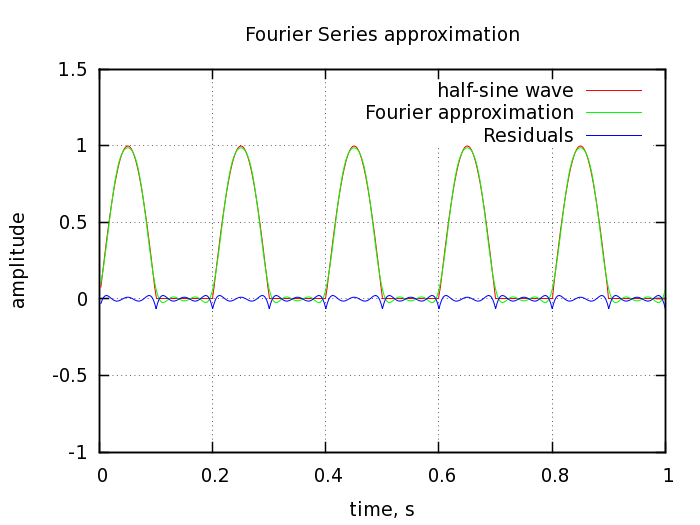
\includegraphics[width=3.75in]{halfsinewave.png}}
\caption{\it \small{Graph of half-sine wave, fourier approximation, and residuals \label{fig1}}}
  \end{center}
\end{figure}

To generate the fourier approximation of the half-sine wave graph a series was summed.  
A four term series had coefficients of: $a0 = \frac{2}{\pi} \approx 0.6366198$\\
entered cosine parameters (in order): [0, -$\frac{2}{3\pi}$, 0, -$\frac{2}{15\pi}$] $\approx$ [0, -0.21221, 0, -0.042441]\\
entered sine parameters (in order): [0.5, 0, 0, 0]

\begin{figure}[H]
  \begin{center}
\centerline{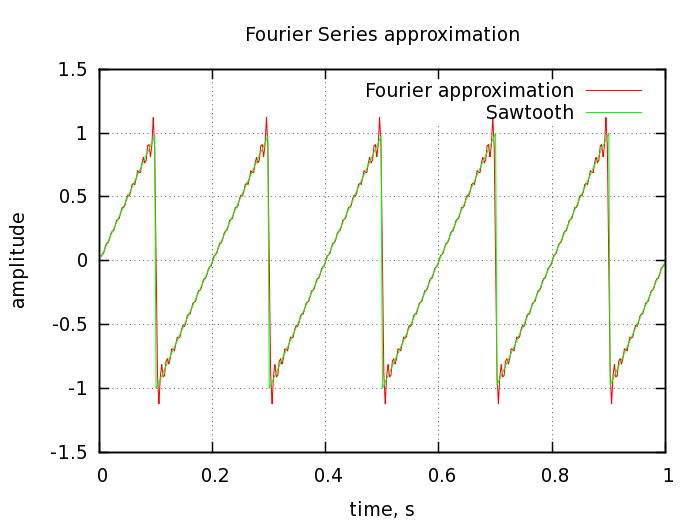
\includegraphics[width=3.75in]{Sawtoothfinal1.png}}
\caption{\it \small{Graph of sawtooth function with fourier approximation \label{fig2}}}
  \end{center}
\end{figure}
To generate the fourier approximation of the sawtooth function a series was summed:
\begin{center}
 $y(t) = \frac{2}{\pi}[sin(\omega t) - \frac{1}{2}sin(2\omega t) + \frac{1}{3}sin(3\omega t) - ... ]$
\end{center}
 ~\\
 ~\\
 ~\\
 ~\\
 ~\\
\begin{figure}[H]
 \centerline{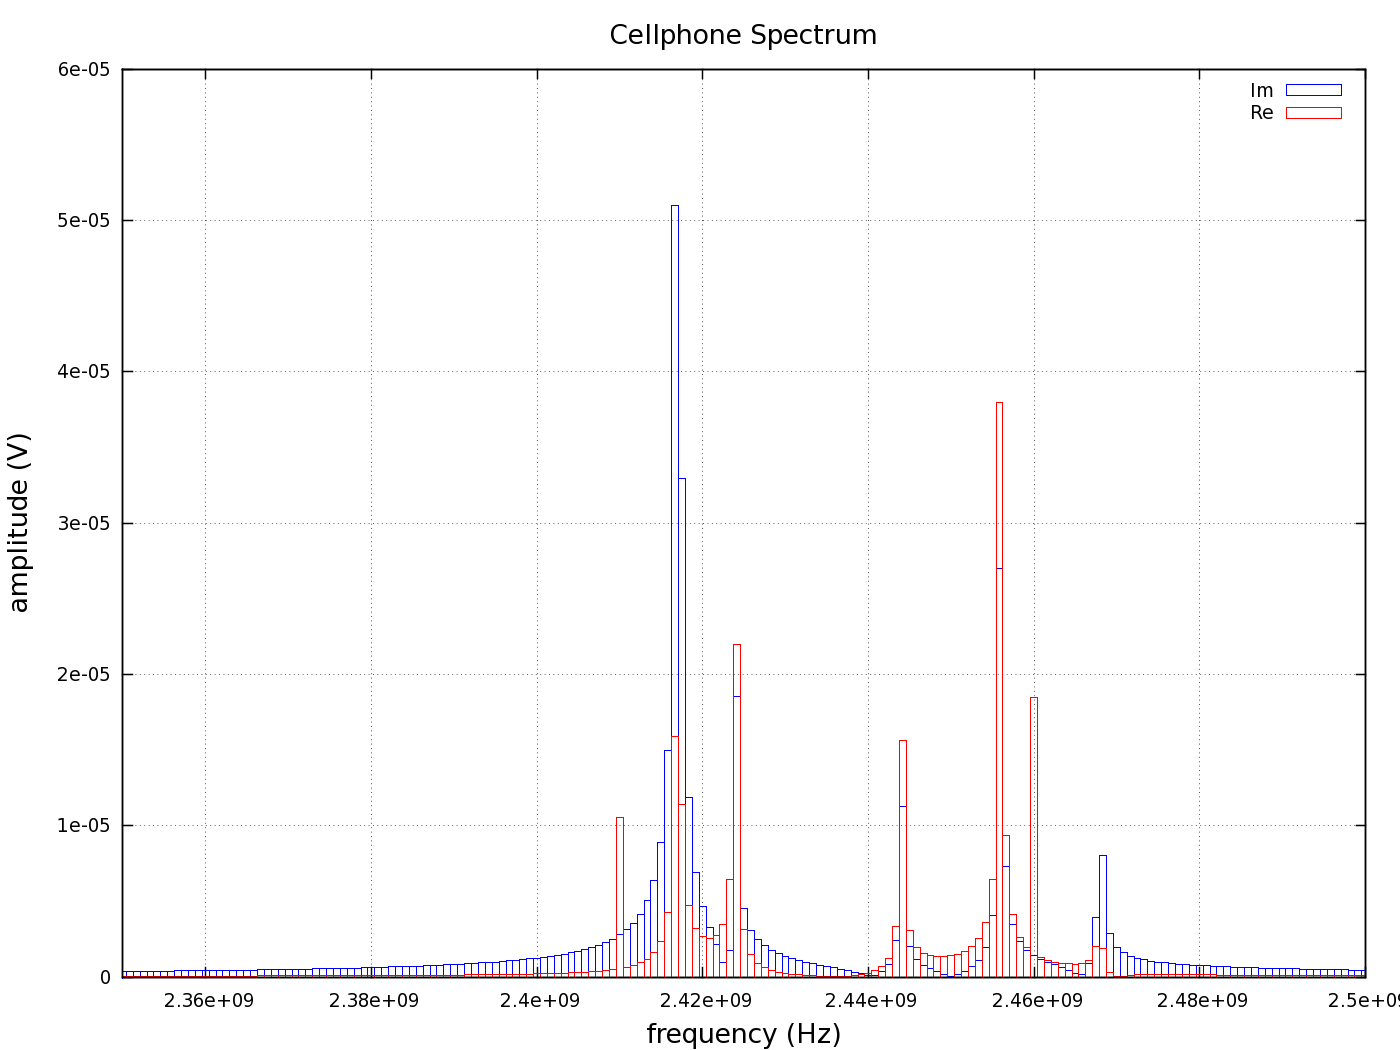
\includegraphics[width=3.5in]{cellphone2.png}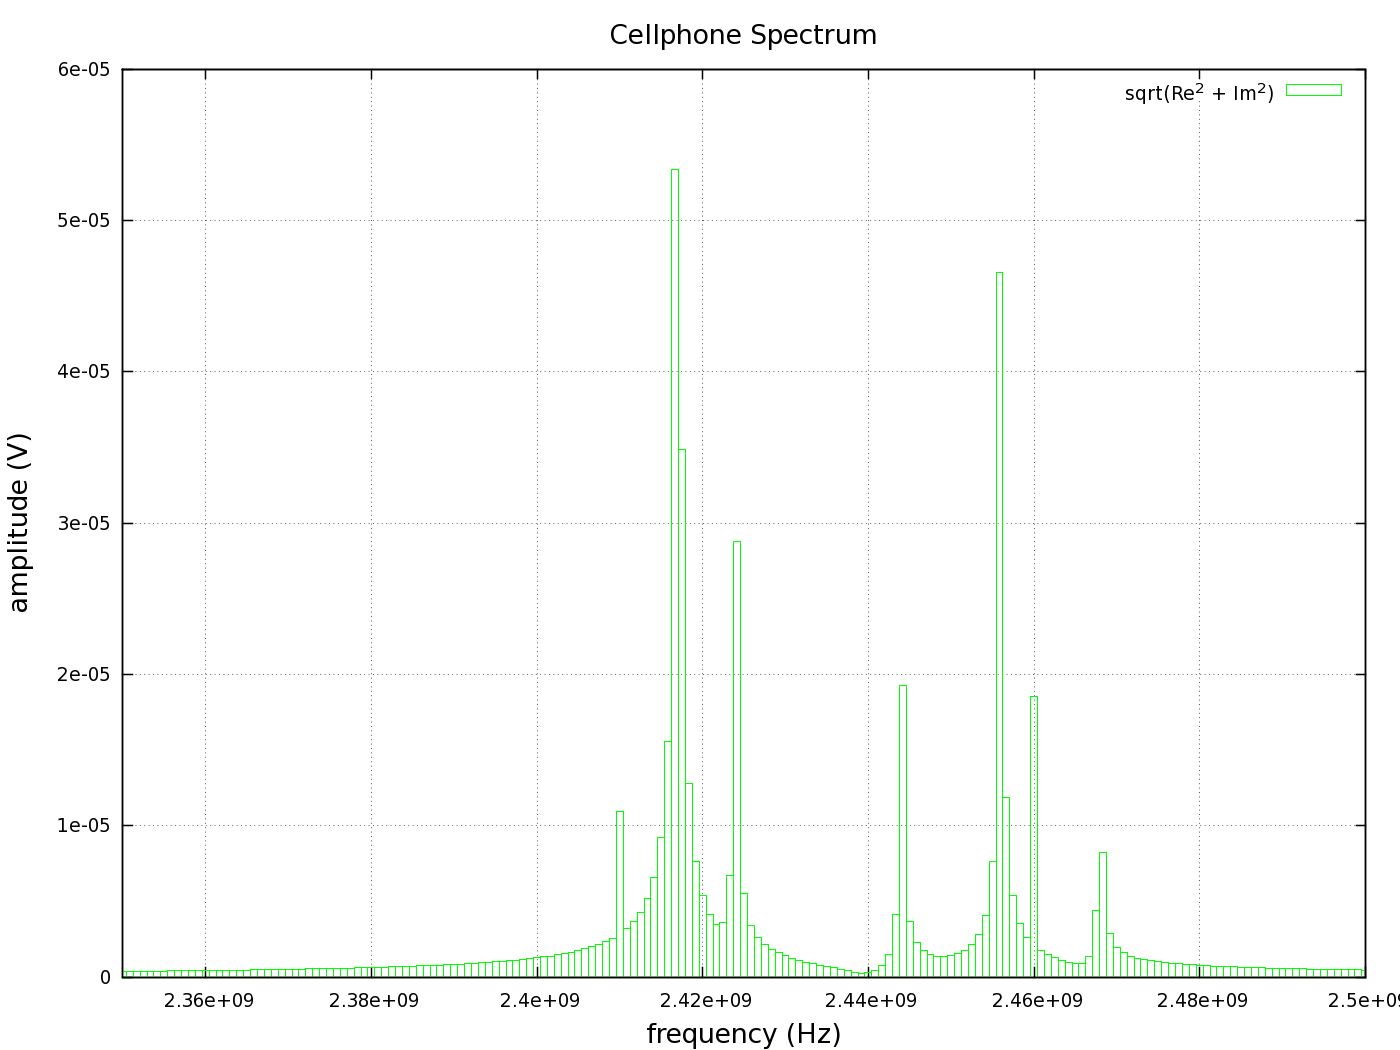
\includegraphics[width=3.5in]{cellphonesquared2.png}}
\caption{\it \small{Discrete fourier transform of cellphone data \label{fig5}}}
\end{figure}
The figure on the left displays the real and imaginary component while the figure on the right graphs the magnitude 
(amplitude) of the fourier component is given by:
\begin{center}
 $\left | A(\omega) \right | ~=~ \sqrt{[Re(F(\omega))]^2 +
            [Im(F(\omega))]^2}$
\end{center}
These figures were generated using the parameters:\\
fmin= 2.3e+09, fmax= 2.5e+09, fstep= 833333\\
120001 lines read, deltat= 1.000000e-11 s, tau = 1.200000e-06 s
 ~\\
 ~\\
 ~\\
 ~\\
 ~\\
%\begin{figure}[H]
%  \begin{center}
%\centerline{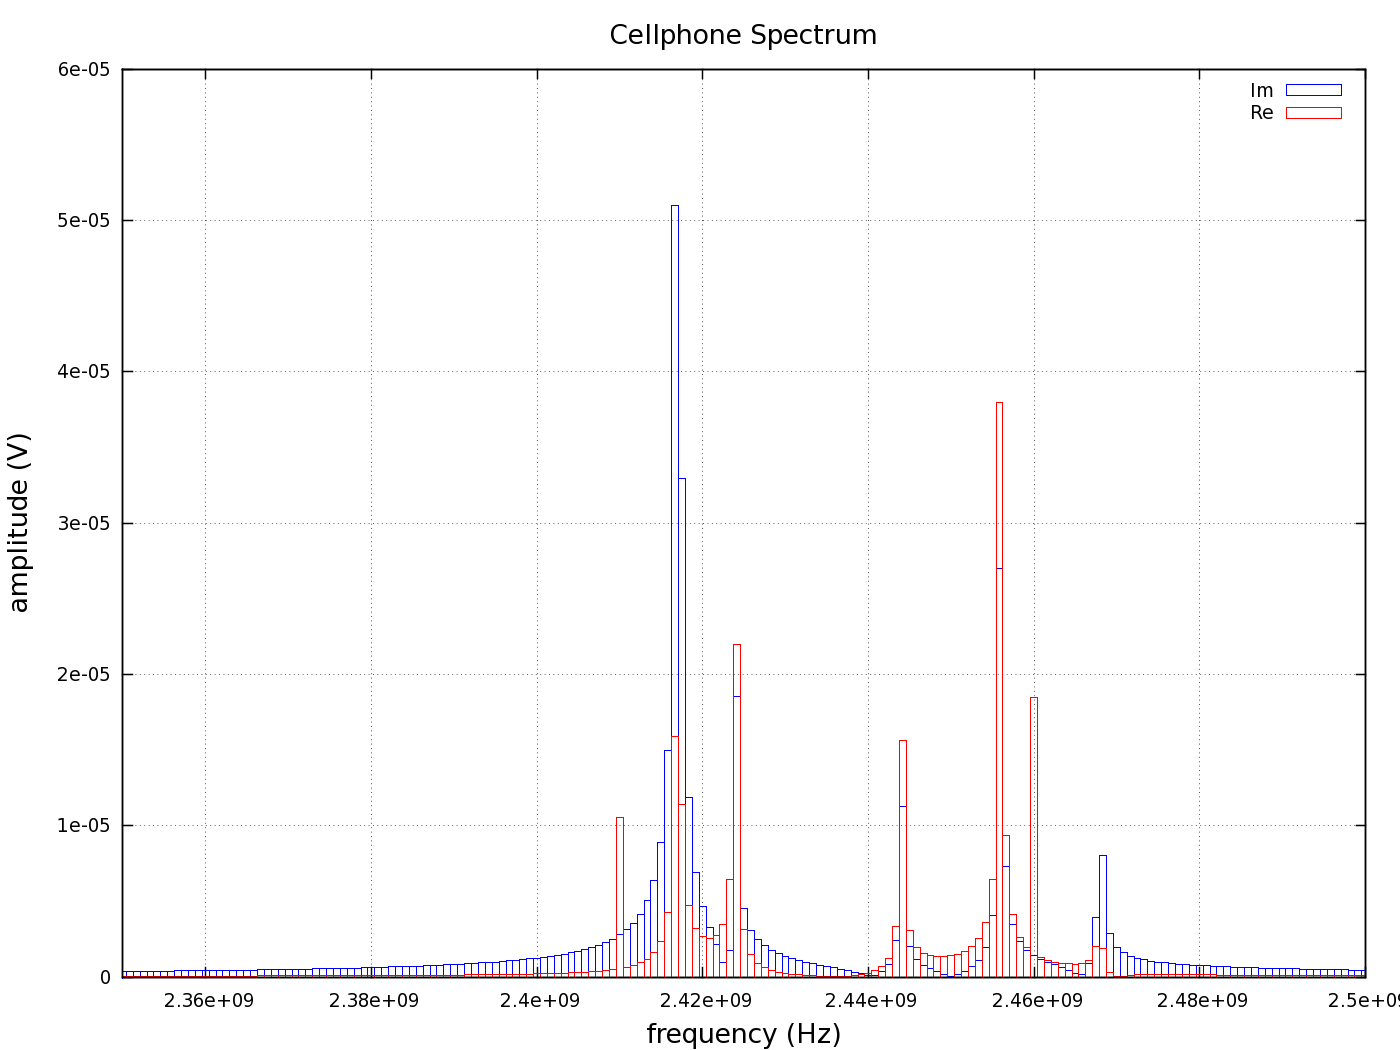
\includegraphics[width=3.75in]{cellphone2.png}}
%\caption{\it \small{Discrete fourier transform of cellphone data \label{fig3}}}
%  \end{center}
%\end{figure}
%Figures 3 and 4 were generated using the parameters:\\
%fmin= 2.3e+09, fmax= 2.5e+09, fstep= 833333\\
%120001 lines read, deltat= 1.000000e-11 s, tau = 1.200000e-06 s
%
%\begin{figure}[H]
%  \begin{center}
%\centerline{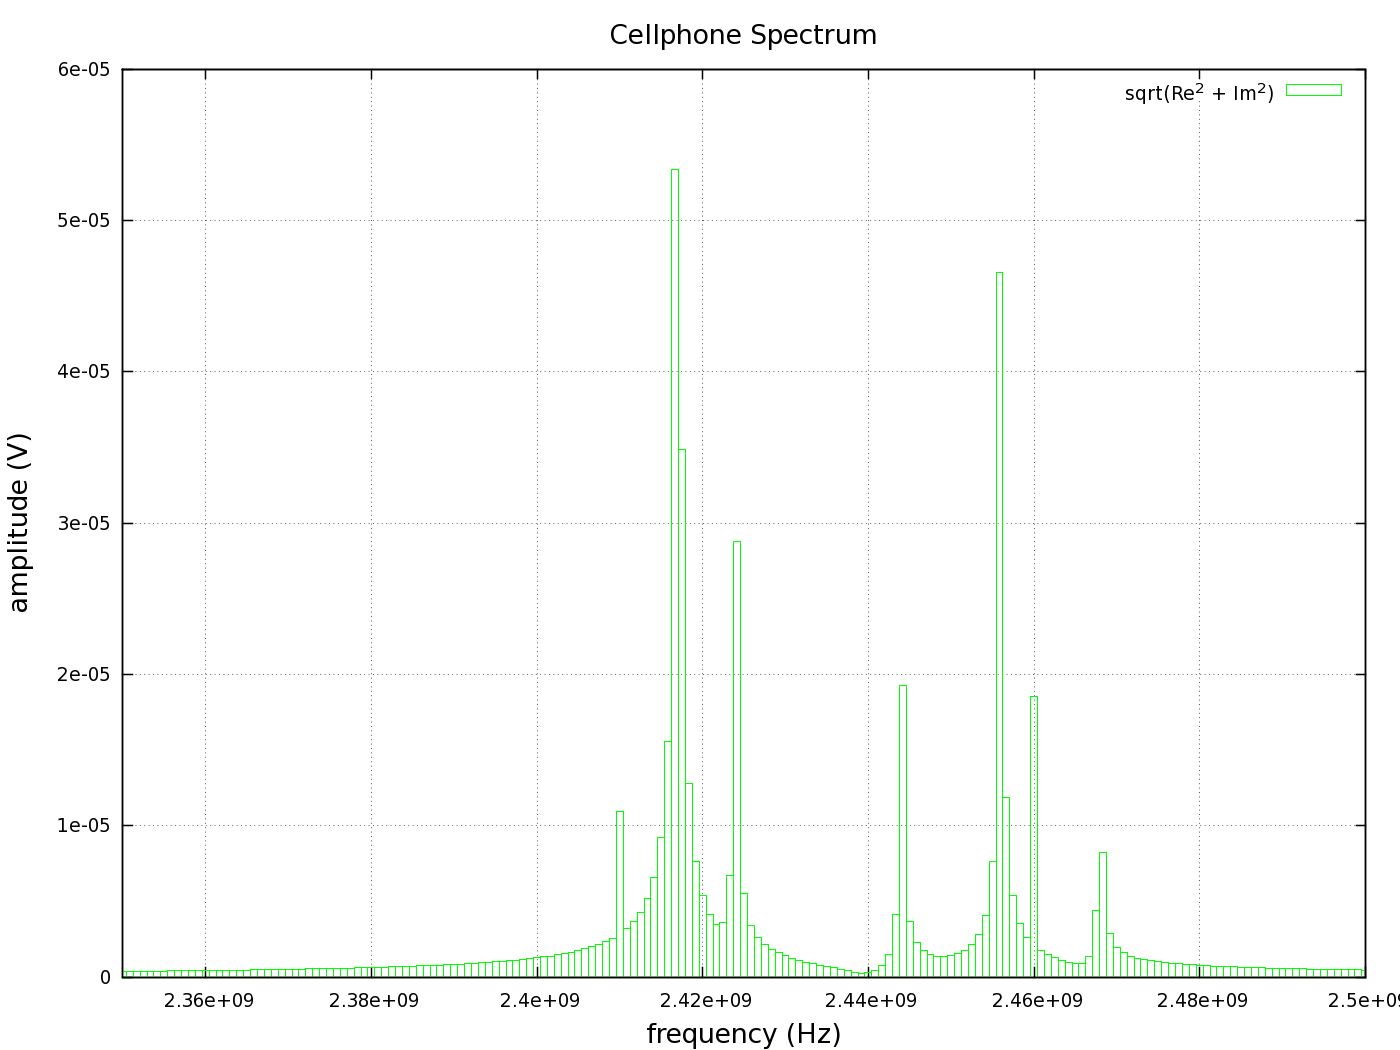
\includegraphics[width=3.75in]{cellphonesquared2.png}}
%\caption{\it \small{Magnitude of the fourier component: cellphone data \label{fig4}}}
%  \end{center}
%\end{figure}
%The magnitude (amplitude) of the fourier component is given by:
%\begin{center}
% $\left | A(\omega) \right | ~=~ \sqrt{[Re(F(\omega))]^2 +
%            [Im(F(\omega))]^2}$
%\end{center}


\begin{figure}[H]
 \centerline{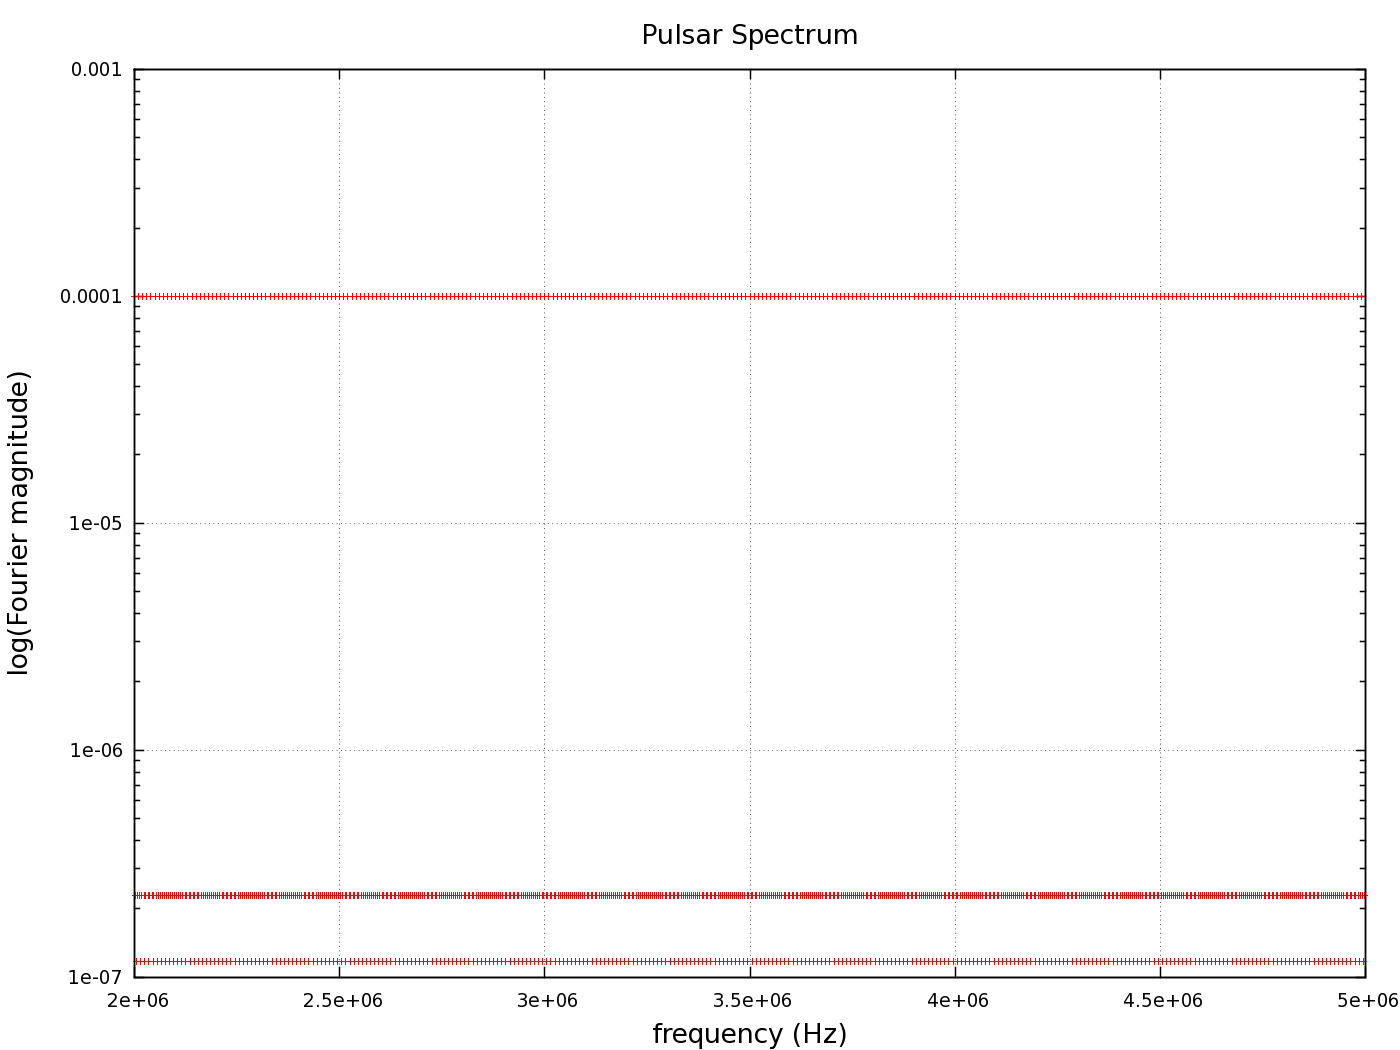
\includegraphics[width=3.5in]{Pulsar12.png}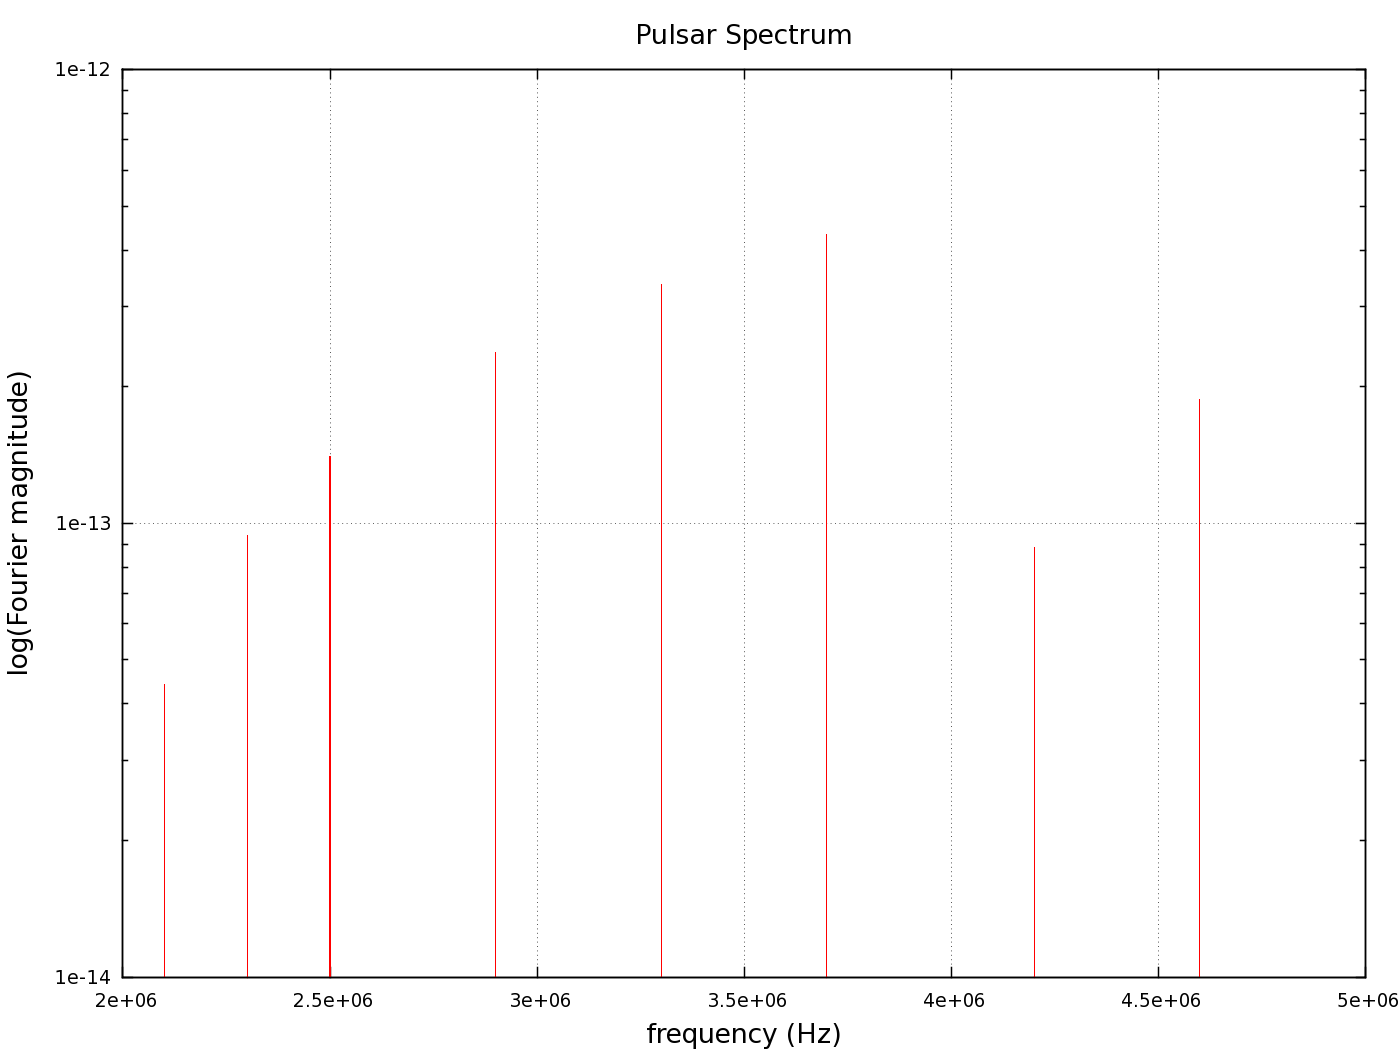
\includegraphics[width=3.5in]{Pulsar22.png}}
\caption{\it \small{Discrete fourier transform of Pulsar data \label{fig5}}}
\end{figure}
The figure on the left was generated using the parameters:\\
fmin= 200000, fmax= 5e+06, fstep= 1000\\
100001 lines read, deltat= 1.000000e-04 s, tau = 1.000000e+01 s



The figure on the right was generated using the parameters:\\
fmin= 200000, fmax= 5e+06, fstep= 100000\\
100001 lines read, deltat= 1.000000e-04 s, tau = 1.000000e+01 s
 ~\\
 ~\\
 ~\\
 ~\\
 ~\\

%\begin{figure}[H]
%  \begin{center}
%\centerline{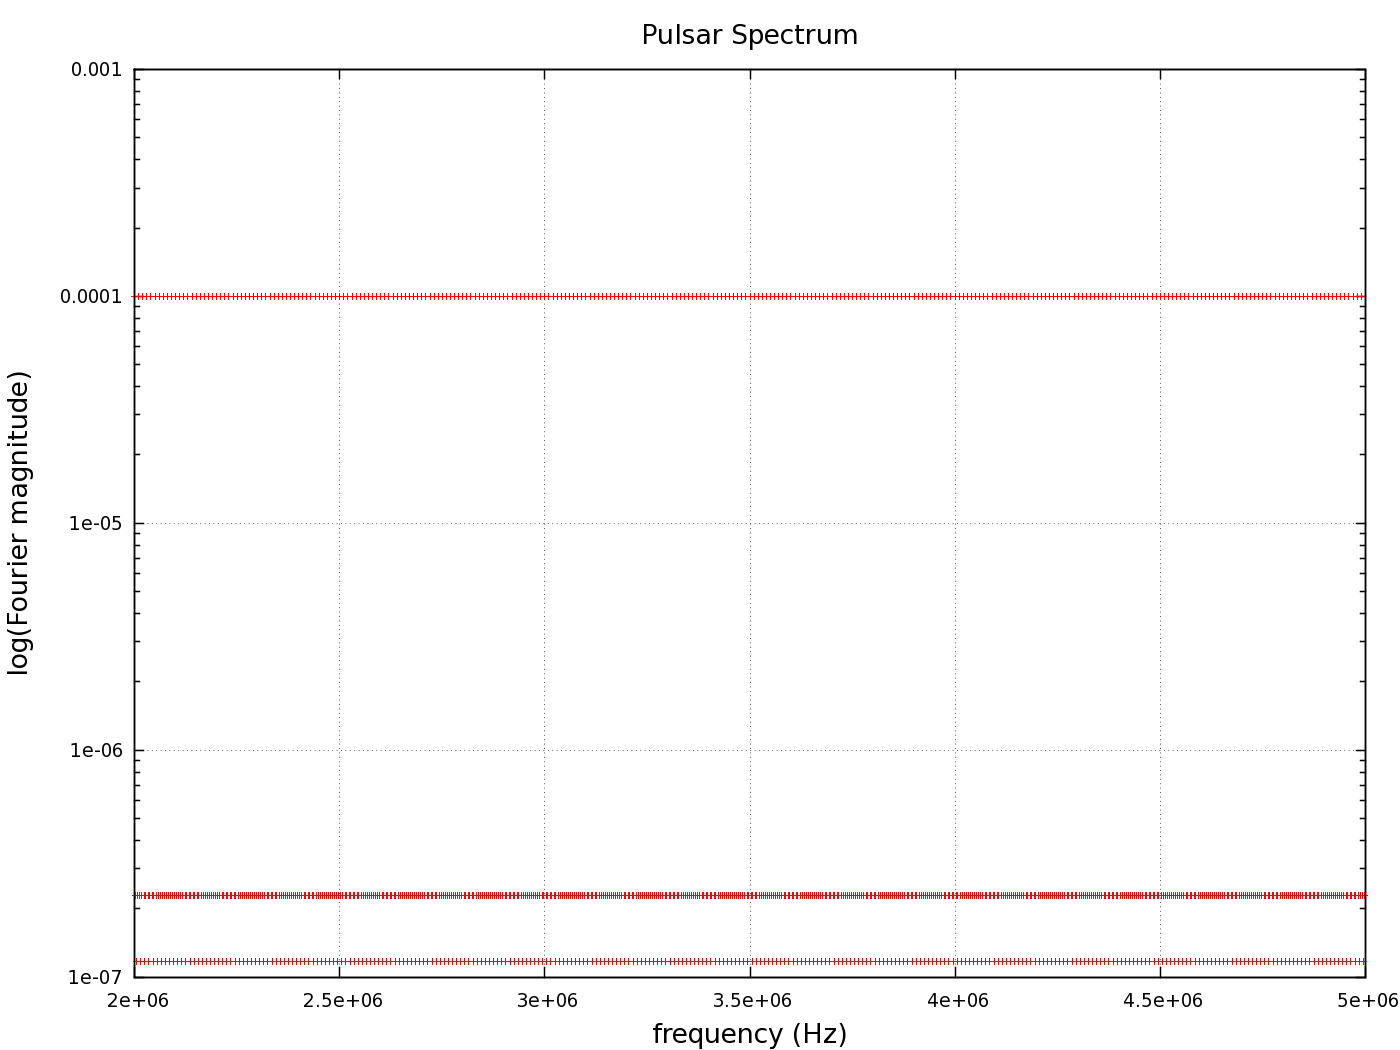
\includegraphics[width=3.75in]{Pulsar12.png}}
%\caption{\it \small{Discrete fourier transform of Pulsar data \label{fig5}}}
%  \end{center}
%\end{figure}
%
%Figure 5 was generated using the parameters:\\
%fmin= 200000, fmax= 5e+06, fstep= 1000\\
%100001 lines read, deltat= 1.000000e-04 s, tau = 1.000000e+01 s
%
%\begin{figure}[H]
%  \begin{center}
%\centerline{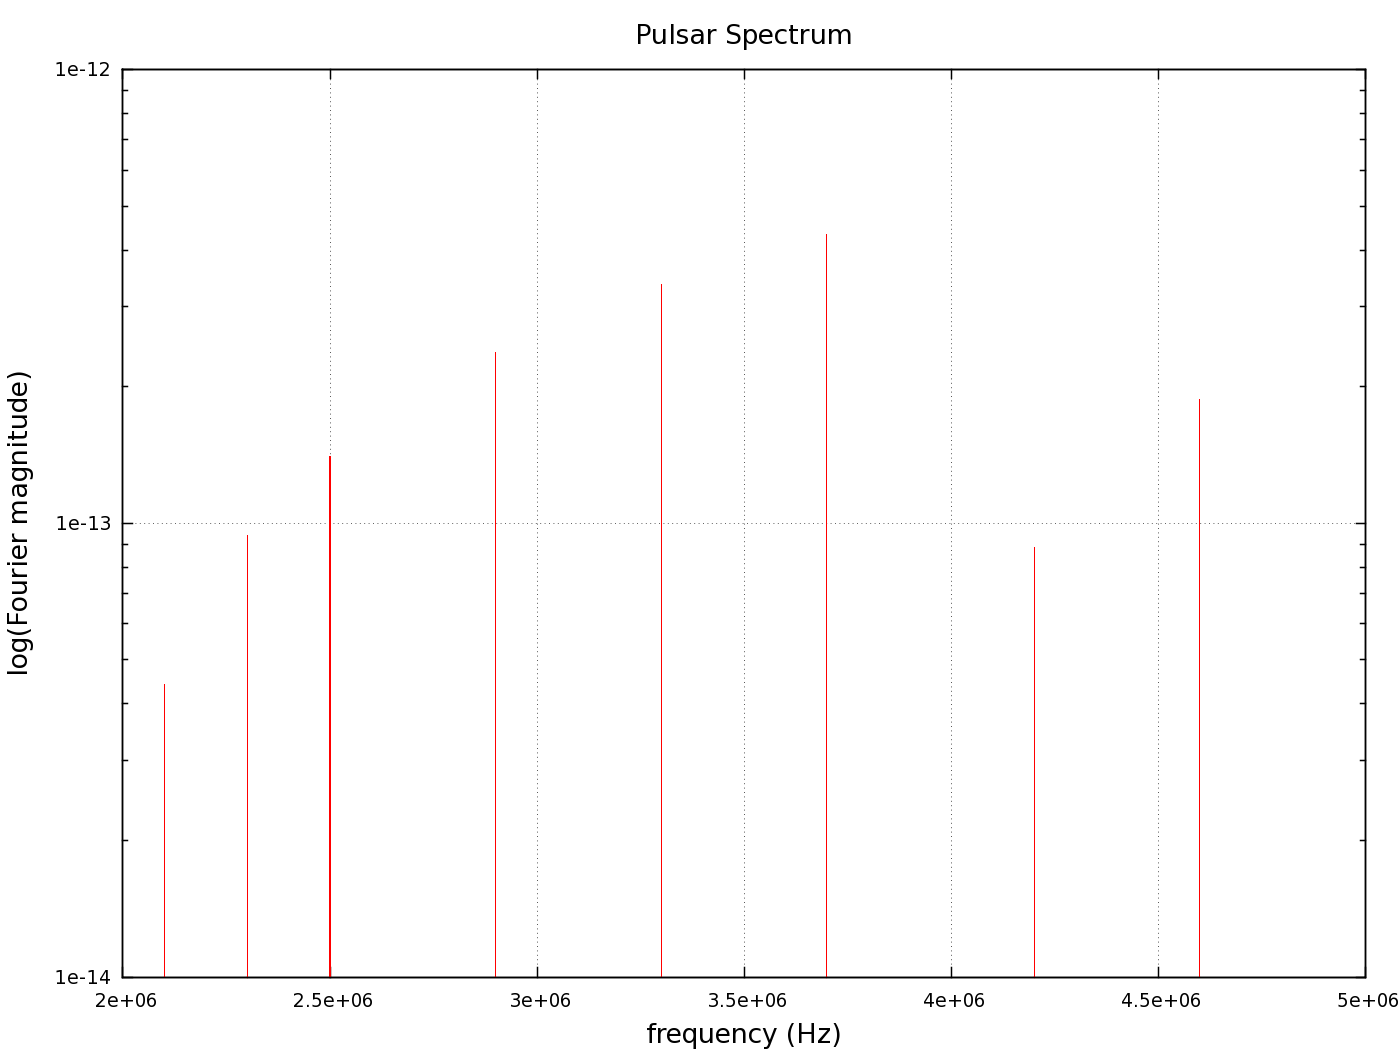
\includegraphics[width=3.75in]{Pulsar22.png}}
%\caption{\it \small{Discrete fourier transform of Pulsar data \label{fig6}}}
%  \end{center}
%\end{figure}
%Figure 6 was generated using the parameters:\\
%fmin= 200000, fmax= 5e+06, fstep= 100000\\
%100001 lines read, deltat= 1.000000e-04 s, tau = 1.000000e+01 s
\begin{figure}[H]
 \centerline{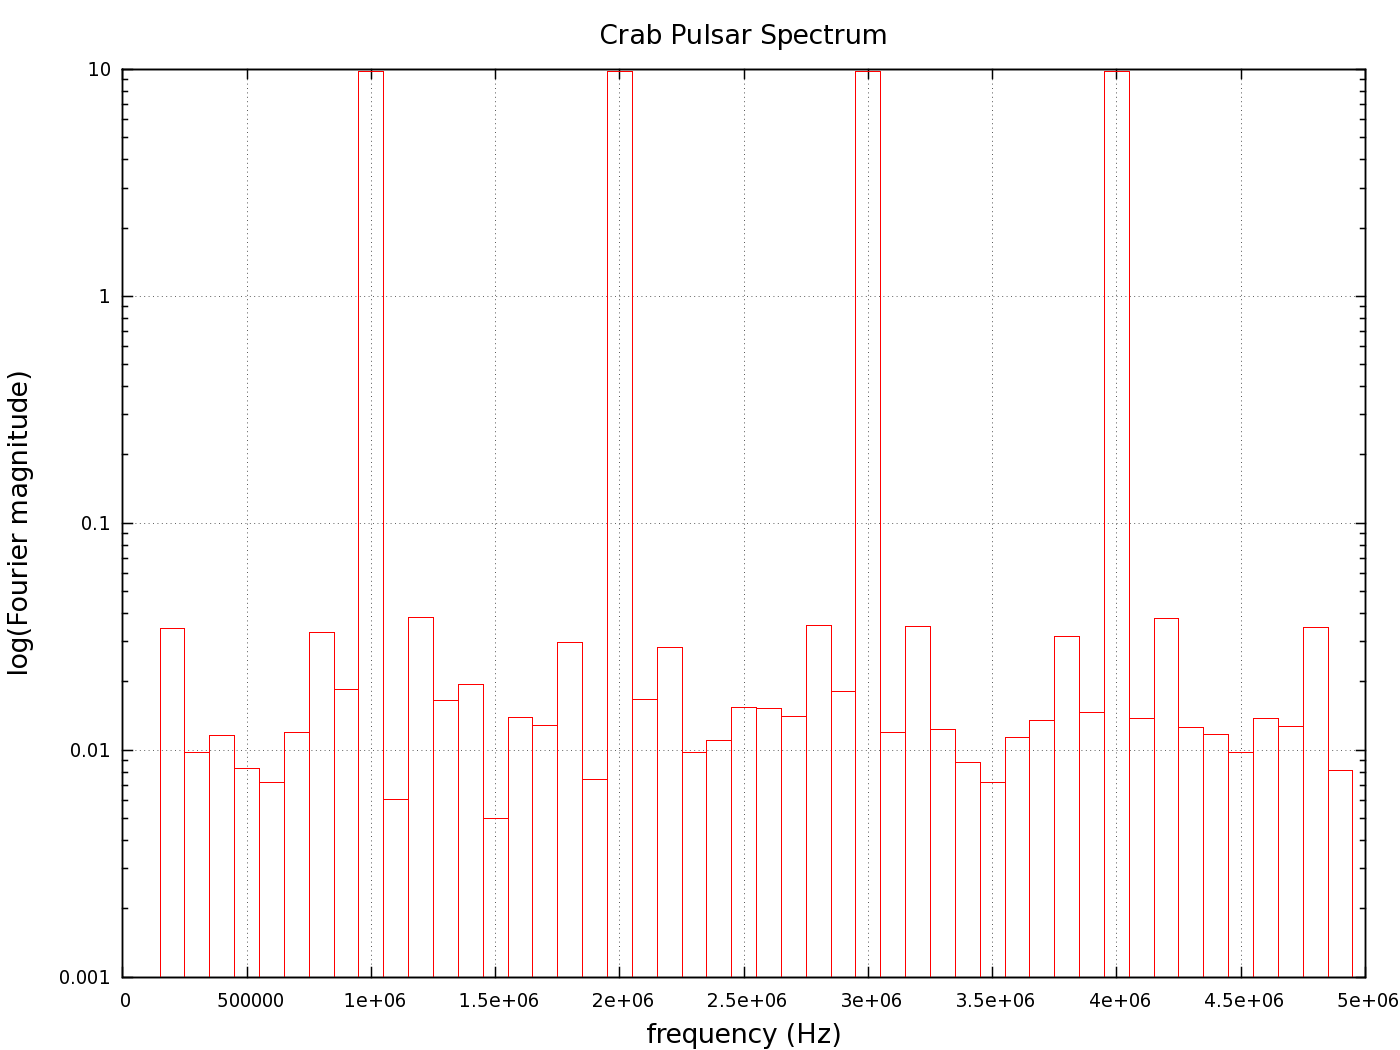
\includegraphics[width=3.5in]{crab.png}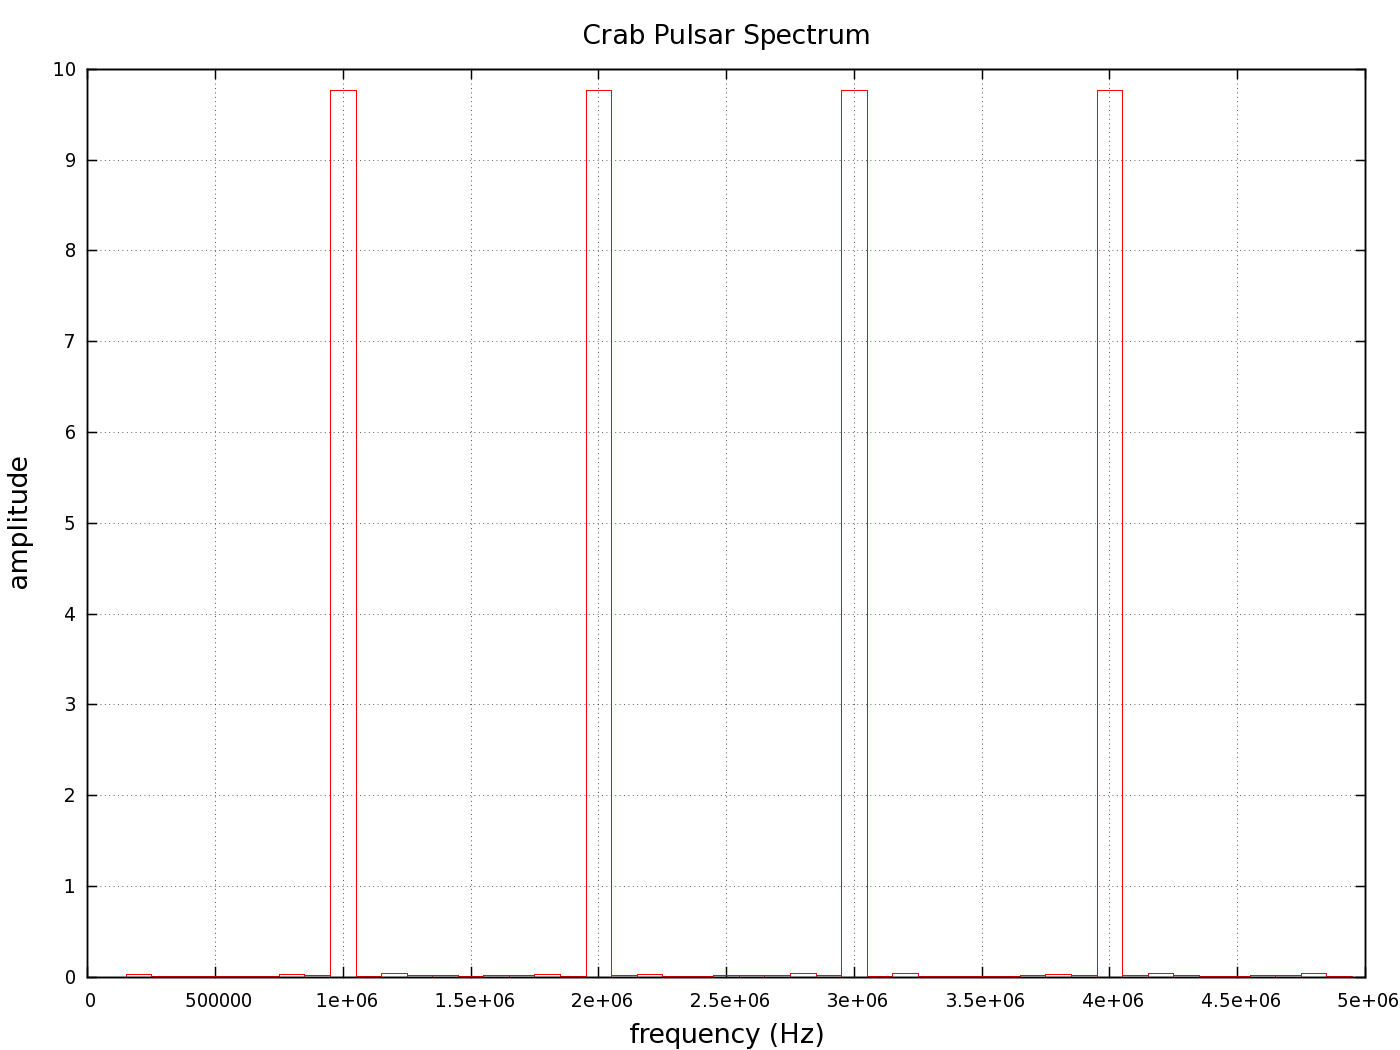
\includegraphics[width=3.5in]{crabnolog.png}}
\caption{\it \small{Discrete fourier transform of Crab Pulsar data \label{fig5}}}
\end{figure}
These figures were generated using the parameters:\\
fmin= 200000, fmax= 5e+06, fstep= 100000\\
148282 lines read, deltat= 6.734000e-05 s, tau = 9.985243e+00 s




\subsection*{}
This report can be seen in color at:\\
\url{http://www2.hawaii.edu/~cmutnik/lab11.pdf}



\end{document}

